\chapter{Experimental procedure}\label{ch:procedure}
In this chapter, the procedure for the experiment is discussed in detail. The experimental procedure starts with calibration of the measuring equipment using a known standard and further using the calibrated equipment to analyze the vortices in the flow.

\section{Calibration of tungsten filament of the bulb}\label{sec:calib bulb}

In this section, the calibration process of tungsten filament is discussed. First, the filament is kept at the middle of the test section and a constant current of 0.310~A is supplied to it (see Fig.~\ref{fig:calibration of filament}). The output of the filament, which is the voltage variation, is recorded in a PC oscilloscope for a time of 5~s without any flow. This data corresponds to no flow condition. The suction fan is then kept at a low speed. The pressure difference in the flow due to the increased speed of the flow is measured using the standard pitot static tube. The corresponding voltage variation in the filament is measured in the PC oscilloscope. Further, the speed of the suction fan is increased and the output is taken both from the pitot static tube and the filament. 
\begin{figure}[H]
    \centering
    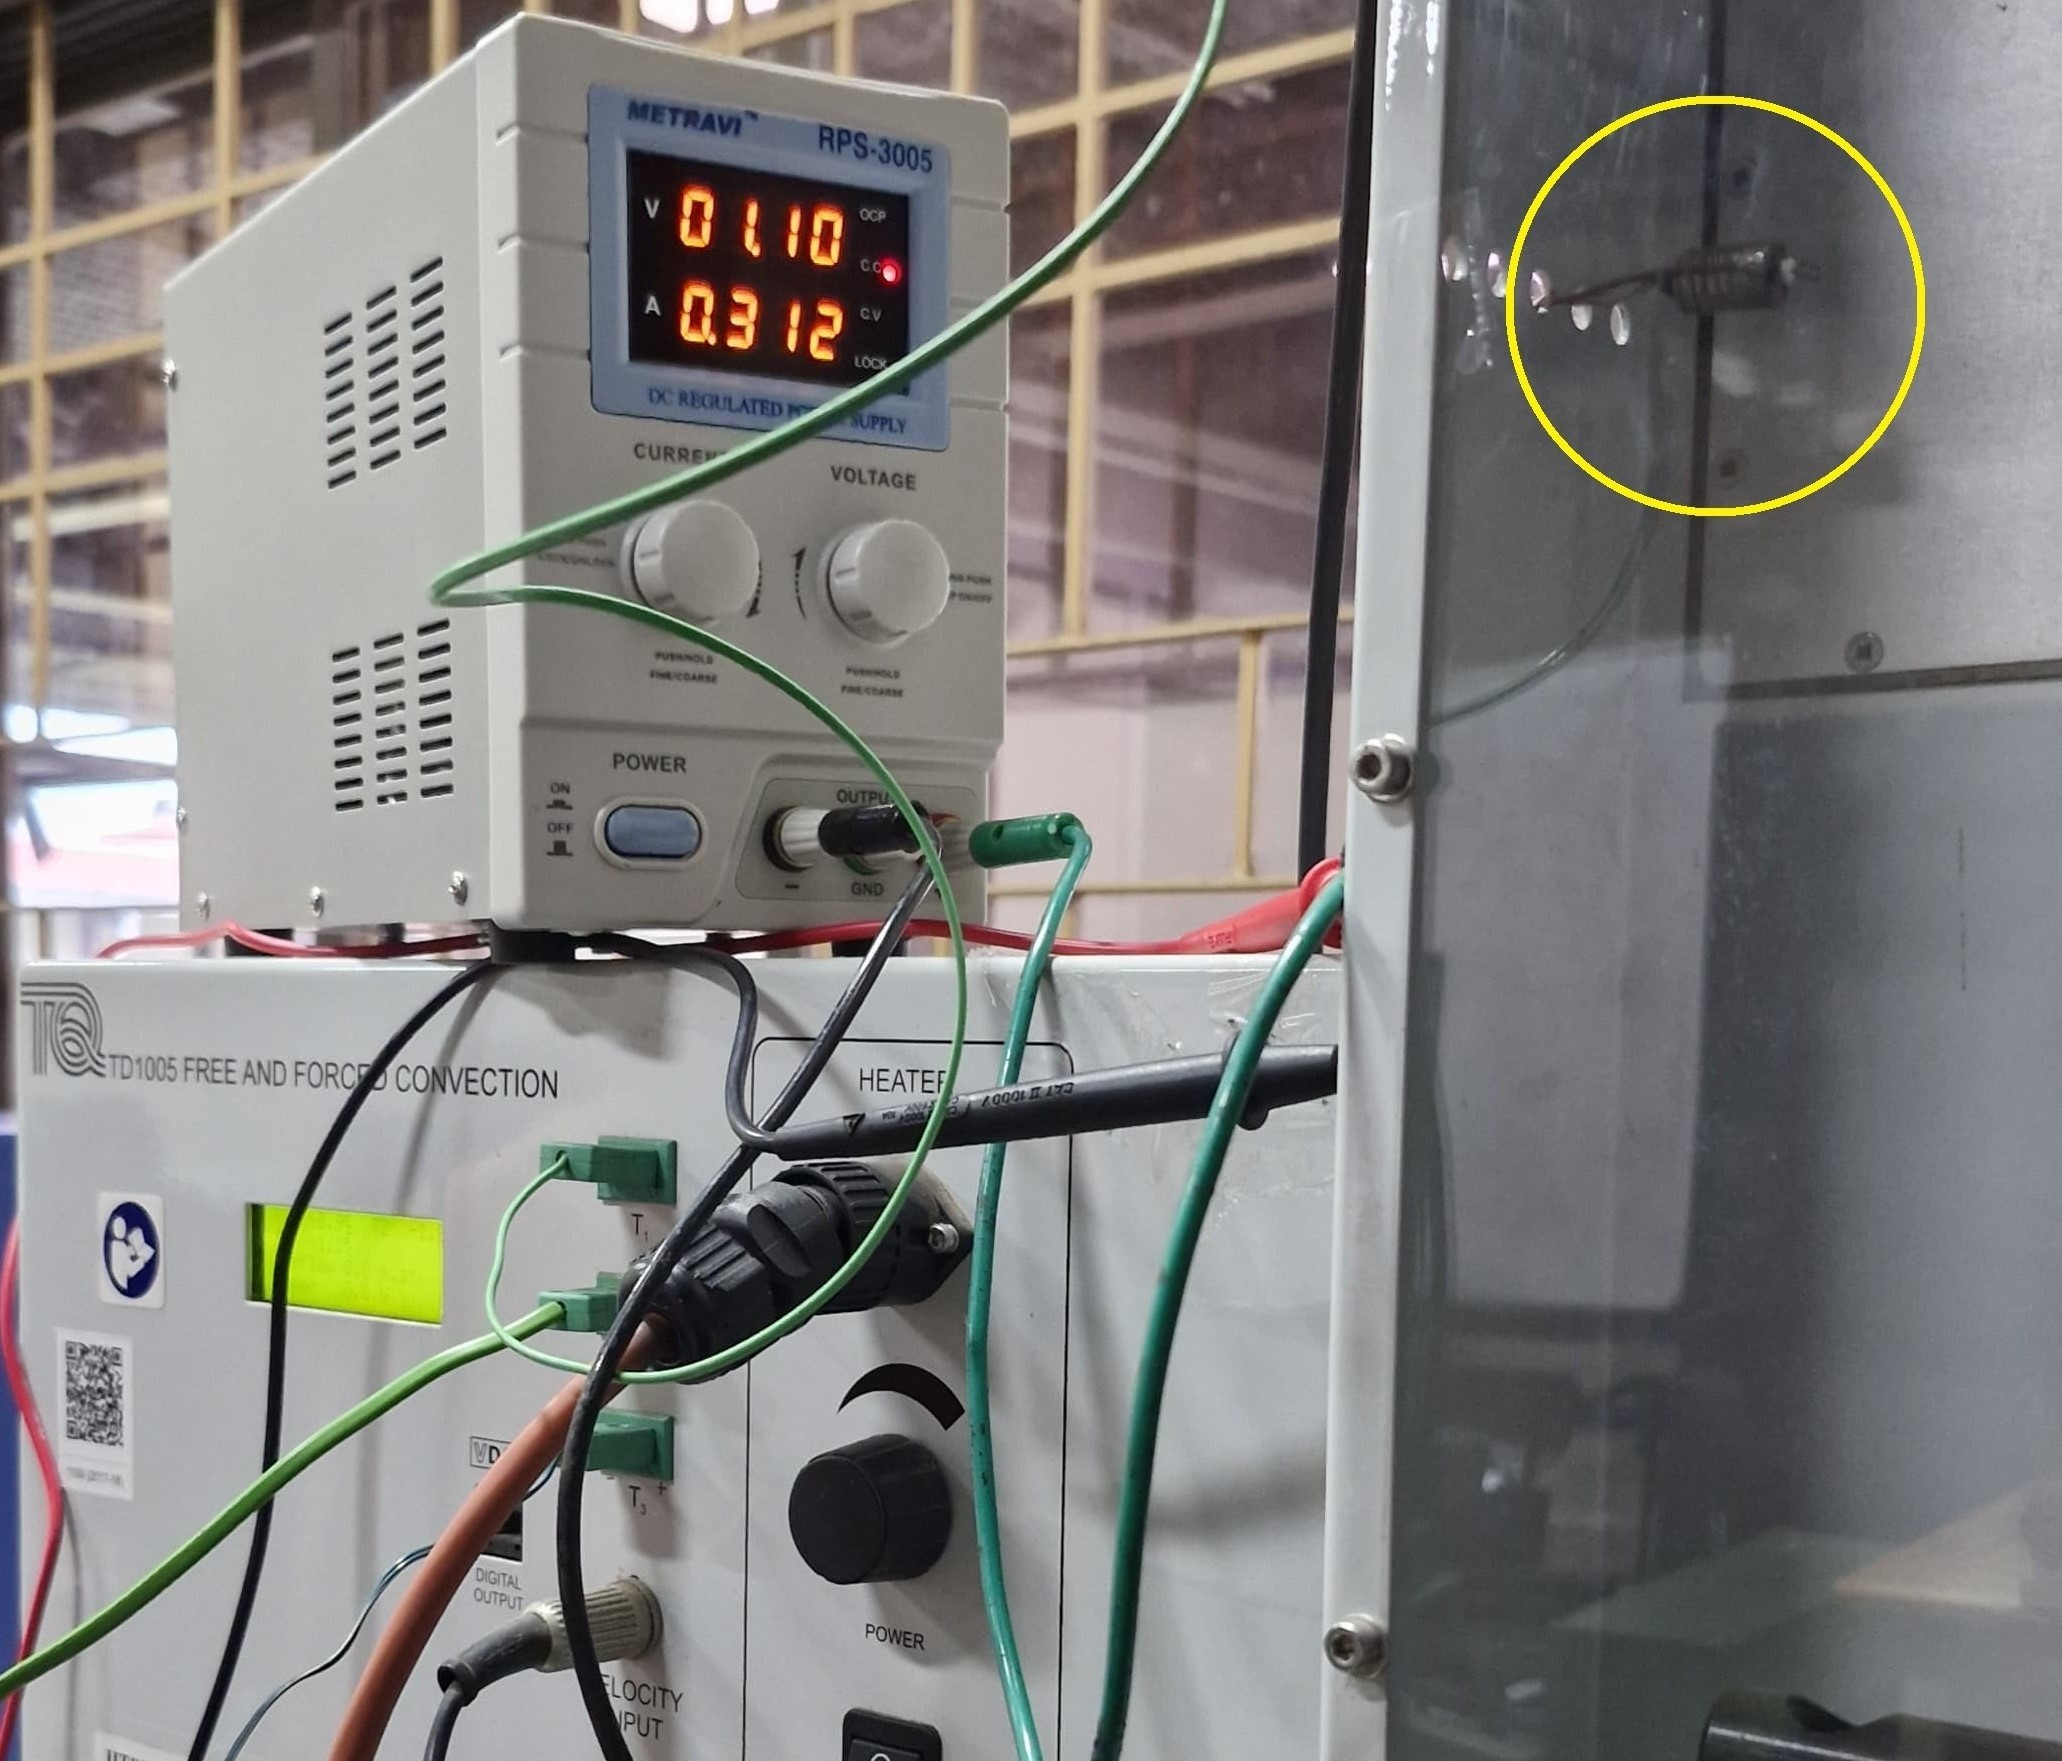
\includegraphics[width=0.7\linewidth]{gfx/TFB_Calibration.jpeg}
    \caption{Calibration of tungsten filament of the bulb}
    \label{fig:calibration of filament}
\end{figure}
\begin{figure}
    \centering
    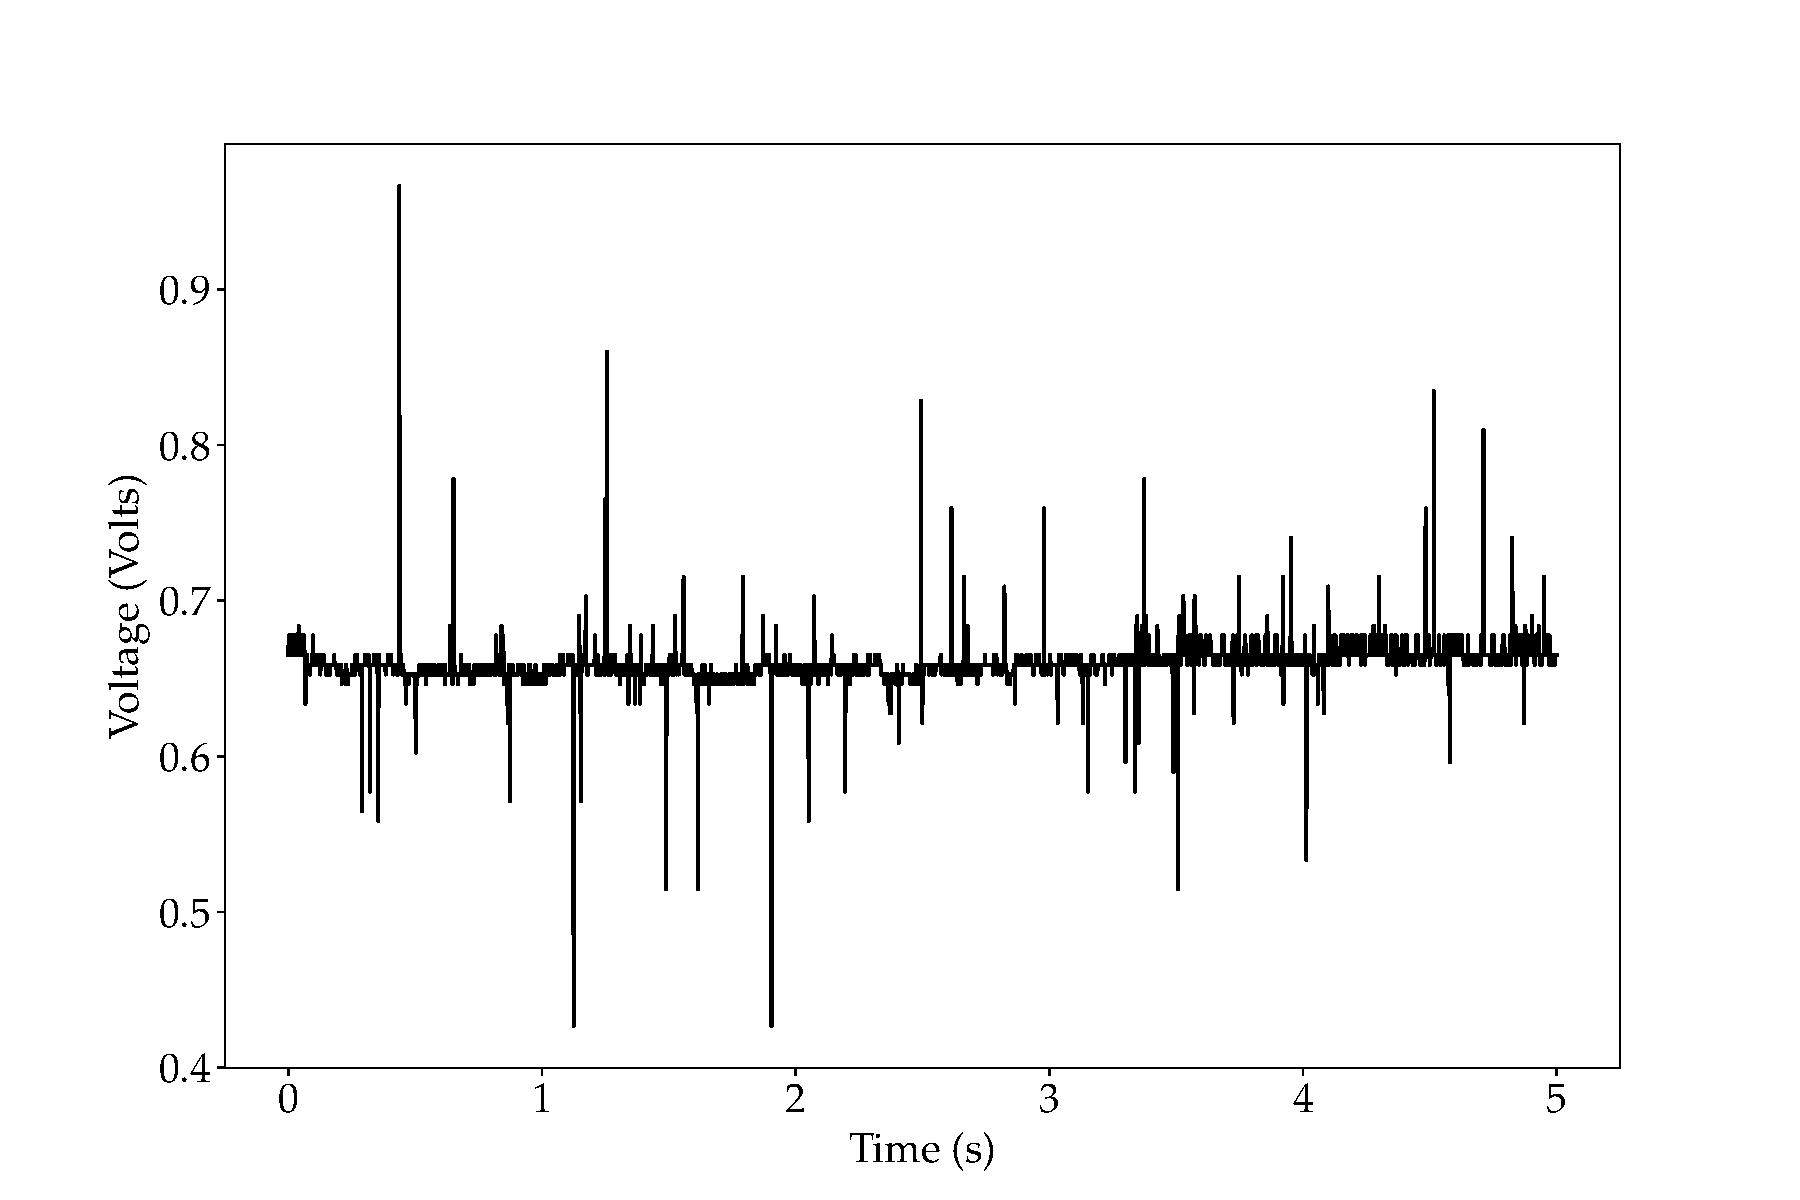
\includegraphics[width=\linewidth]{gfx/Voltage_vs_time_for_4Pa.pdf}
    \caption{Voltage variation with time for a flow having pressure of 4~Pa recorded in a PC oscilloscope.}
    \label{fig:V_t_calib bulb 4 Pa}
\end{figure}

The output voltage of the filament measured from the oscilloscope for a pitot tube pressure of 4~Pa is given in Fig.~\ref{fig:V_t_calib bulb 4 Pa}. From the figure, it can be seen that there are fluctuations in the voltage. For calculation purposes, the mean value of the voltage fluctuation is considered. The same procedure is followed for other flow velocities. The filament output voltage is recorded for a pitot tube pressure of 1~Pa, 2~Pa, 3~Pa, 4~Pa, 6~Pa, 9~Pa, 12~Pa, 14~Pa, 17~Pa, 19~Pa and 24~Pa. The flow velocity corresponding to pitot static tube pressure is calculated using Eq.~(\ref{eq:press_vel equation}).
\begin{equation}\label{eq:press_vel equation}
    U = \sqrt{\frac{2\Delta P}{\rho}},
\end{equation}
where $\Delta P$ is the differential pressure measured in the pitot static tube and $\rho$ is the density of air (= 1.21 $kg/m^3$). The differential pressure, velocity, and corresponding voltage output of the filament is given in Table~\ref{tab:output_bulb filament}. 
\begin{table}
$E_0 = 1.09~V$
    \centering
    \caption{The flow velocity and the output mean voltage of the tungsten filament of the bulb.}
    \begin{tabular}{|c|c|c|}
    \toprule
       \textbf{Differential Pressure $\Delta P$ (Pa)}  & \textbf{Velocity $U$ (m/s)} & \textbf{Mean Voltage $E$ (Volts)} \\
       \midrule
        1 & 1.307 & 0.842 \\ \hline
        2 & 1.849 & 0.756 \\ \hline
        3 & 2.265 & 0.689 \\ \hline
        4 & 2.615 & 0.659 \\ \hline
        6 & 3.203 & 0.641 \\ \hline
        9 & 3.922 & 0.653 \\ \hline
        12 & 4.529 & 0.621 \\ \hline
        14 & 4.892 & 0.596 \\ \hline
        17 & 5.391 & 0.642 \\ \hline
        19 & 5.699 & 0.599 \\ \hline
        24 & 6.405 & 0.561 \\ 
        \bottomrule
    \end{tabular}
    \label{tab:output_bulb filament}
\end{table}
The tungsten filament is then calibrated by applying the output from the pitot tube into King's law,
\begin{equation}\label{eq:kings law}
    E^2 = E_0^2 - BU^n,
\end{equation}
where $E$ is the measured mean output voltage, $E_0$ is the mean voltage corresponding to no flow condition, $U$ is the flow velocity. $B$ and $n$ are numerical constants that can be estimated by regression analysis while calibrating the filament. Equation.~(\ref{eq:kings law}) is an exponential function that can be linearized by taking logarithms. Rearranging and taking natural log on both sides of Eq.~(\ref{eq:kings law}) gives 
\begin{equation}\label{eq:linearized kings law}
    \ln{(E_0^2-E^2)} = n\ln{U} + \ln{B}.
\end{equation}
Equation~(\ref{eq:linearized kings law}) is the linearized form of King's law and can be expressed in the form $y = mx + c$. The linearized King's law equation can be solved using the method of least squares to find the numerical constants $B$ and $n$. The solution steps for method of least squares is given by
\begin{align}
    & \Sigma \ln{(E_0^2-E^2)} = n\Sigma \ln{U} + q\ln{B}\label{eq:lin eq 1}\\ 
    & \Sigma (\ln{(E_0^2-E^2)}\times \ln{U}) = n \Sigma (\ln{U})^2 + \ln{B}~ \Sigma\ln{U}\label{eq:lin eq 2},
\end{align}
where $q$ is the number of sample spaces. The above two equations are the system of linear equations in two variables which can be solved directly and the constants $B$ and $n$ can be calculated. When solving the equations using Table \ref{tab:output_bulb filament}, the constants $B$ and $n$ are estimated as 0.512 and 0.299, respectively. So the calibration equation is given by
\begin{equation}\label{eq:calib_eqn_filament}
    E^2 = 1.188 - 0.512\cdot U^{0.299.}.
\end{equation}
\begin{table}[H]
    \centering
    \caption{The difference of calibrated voltage from measured voltage for filament of the bulb.}
    \begin{tabular}{|c|c|c|c|}
    \toprule
         Measured $E^2$& Calculated $E^2$ & Error & Error$^2$\\
         \midrule
          0.708 & 0.635 & 0.073 & 5.34$\times$10$^{-3}$ \\ \hline
          0.571 & 0.575 & -0.003 & 1.14$\times$10$^{-5}$ \\ \hline
          0.474 & 0.536 & -0.062 & 3.88$\times$10$^{-3}$ \\ \hline
          0.435 & 0.508 & -0.073 & 5.33$\times$10$^{-3}$ \\ \hline
          0.411 & 0.465 & -0.055 & 2.99$\times$10$^{-3}$ \\ \hline
          0.426 & 0.420 & 0.006 & 3.68$\times$10$^{-5}$ \\ \hline
          0.386 & 0.386 & -0.001 & 3.58$\times$10$^{-7}$ \\ \hline
          0.355 & 0.368 & -0.013 & 1.66$\times$10$^{-4}$ \\ \hline
          0.412 & 0.343 & 0.068 & 4.68$\times$10$^{-3}$ \\ \hline
          0.359 & 0.329 & 0.029 & 8.57$\times$10$^{-4}$ \\ \hline
          0.315 & 0.299 & 0.016 & 2.58$\times$10$^{-4}$ \\
         \bottomrule
         
    \end{tabular}
    \label{tab:error_filament_bulb}
\end{table}
\begin{figure}[H]
    \centering
    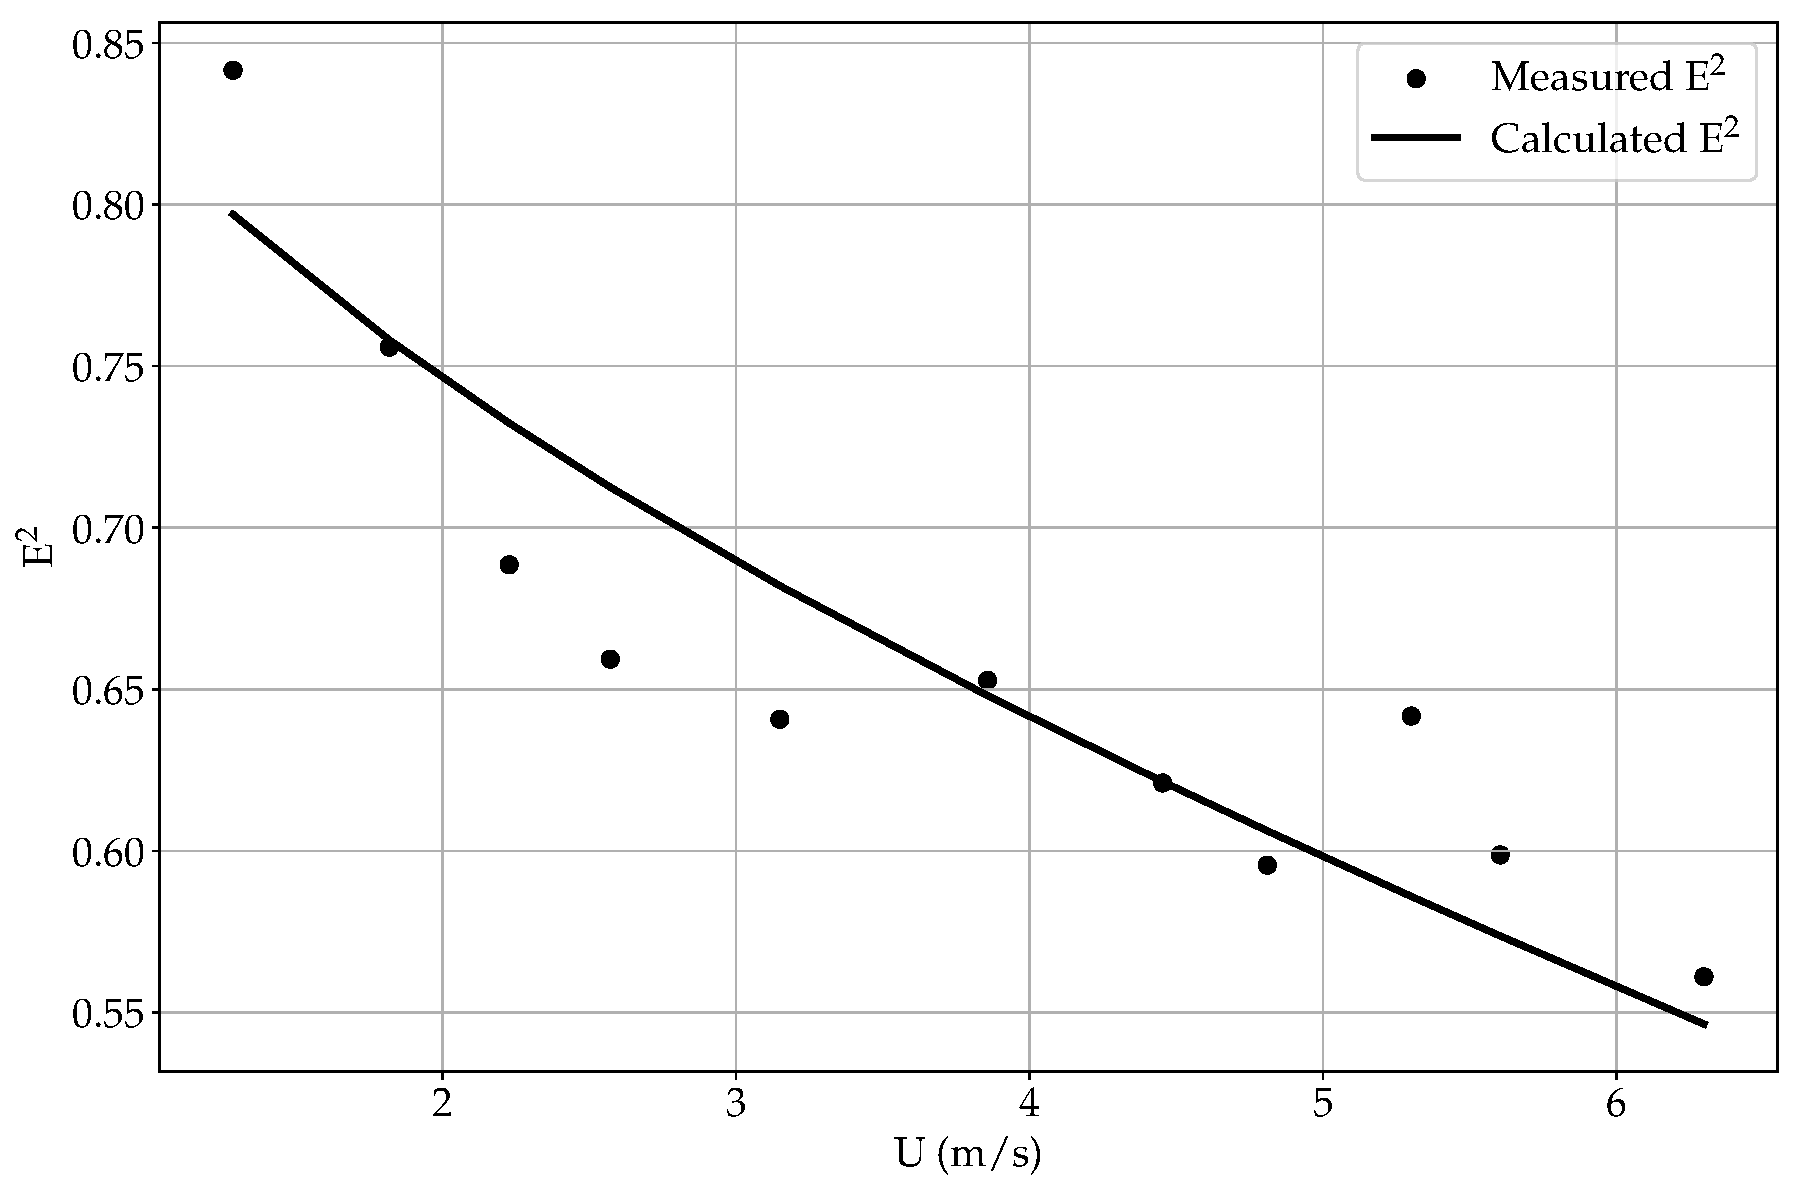
\includegraphics[width=\linewidth]{gfx/calibration_of_bulb_filament.pdf}
    \caption{Comparison of measured voltage and Calculated voltage of the filament of a bulb.}
    \label{fig:Calib_curv_filament}
\end{figure}
The velocity of the flow is substituted back in Eq.~(\ref{eq:calib_eqn_filament}) and the voltage is calculated. The error between the measured and calculated voltages is estimated and is given in Table~\ref{tab:error_filament_bulb}. The comparison between the measured and calculated voltages is given in Fig.~\ref{fig:Calib_curv_filament}. It can be seen that the voltage decreases with an increase in the velocity. When current is supplied to the wire, it will heat up. Due to the increase in heat, the resistance of the wire increases. Now when air flows across the wire, it is cooled by convection and thus its resistance also decreases. So, to maintain the same current on the wire, the voltage across the wire decreases. 

The standard deviation $\sigma$ can be calculated using the equation
\begin{equation}
    \sigma = \sqrt{\frac{\Sigma Error^2}{q}} = 0.0463\\ \text{and}\\
    3\sigma = 0.1388
\end{equation}
The calibration equation for the tungsten filament of the bulb is given by
\begin{equation}
    E^2 = 1.188 - 0.512\cdot U^{0.299} \pm 0.1388
\end{equation}

\section{Time constant of the filament of the bulb}

The time constant $\tau$ of a sensor is the time taken to produce a steady output when a step input is given to it. The suction fan is kept at a known speed.
\begin{figure}[ht]
    \centering
    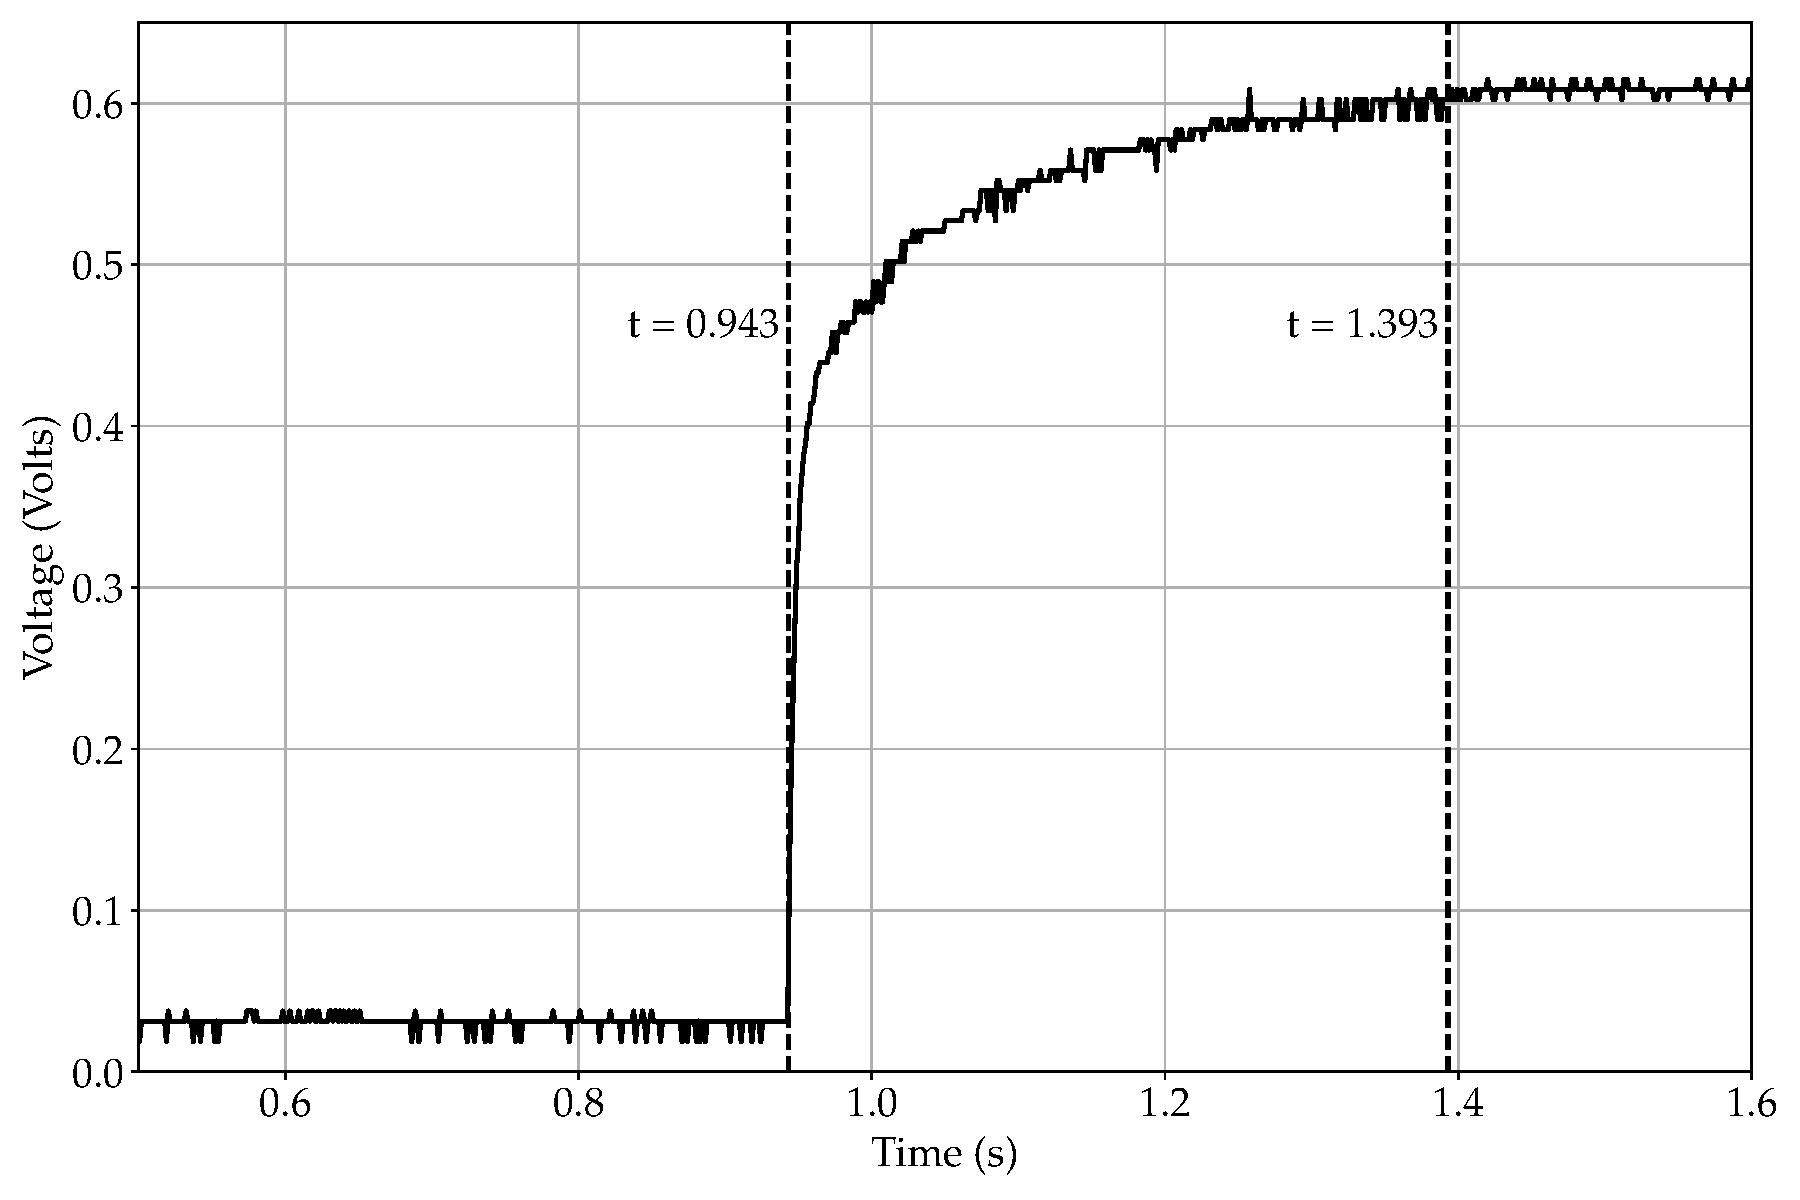
\includegraphics[width=\linewidth]{gfx/Time_constant_bulb.pdf}
    \caption{Response of the tungsten filament of the bulb to the step input.}
    \label{fig:time_filament}
\end{figure}
The bulb filament is kept inside the test section. The output voltage is then recorded in the oscilloscope. The input constant current is supplied instantaneously to the filament. The sudden increase in the voltage is also recorded in the oscilloscope. The time taken to reach the maximum steady voltage from the minimum is called the time constant. Figure~\ref{fig:time_filament} shows the variation of the output voltage with time when input is given instantaneously to the filament. It can be seen from Fig.~\ref{fig:time_filament} that the filament approximately takes about 450~ms to give steady output when a step input is applied.




\section{Calibration of Hot wire anemometer}
% \begin{figure}[ht]
%     \centering
%     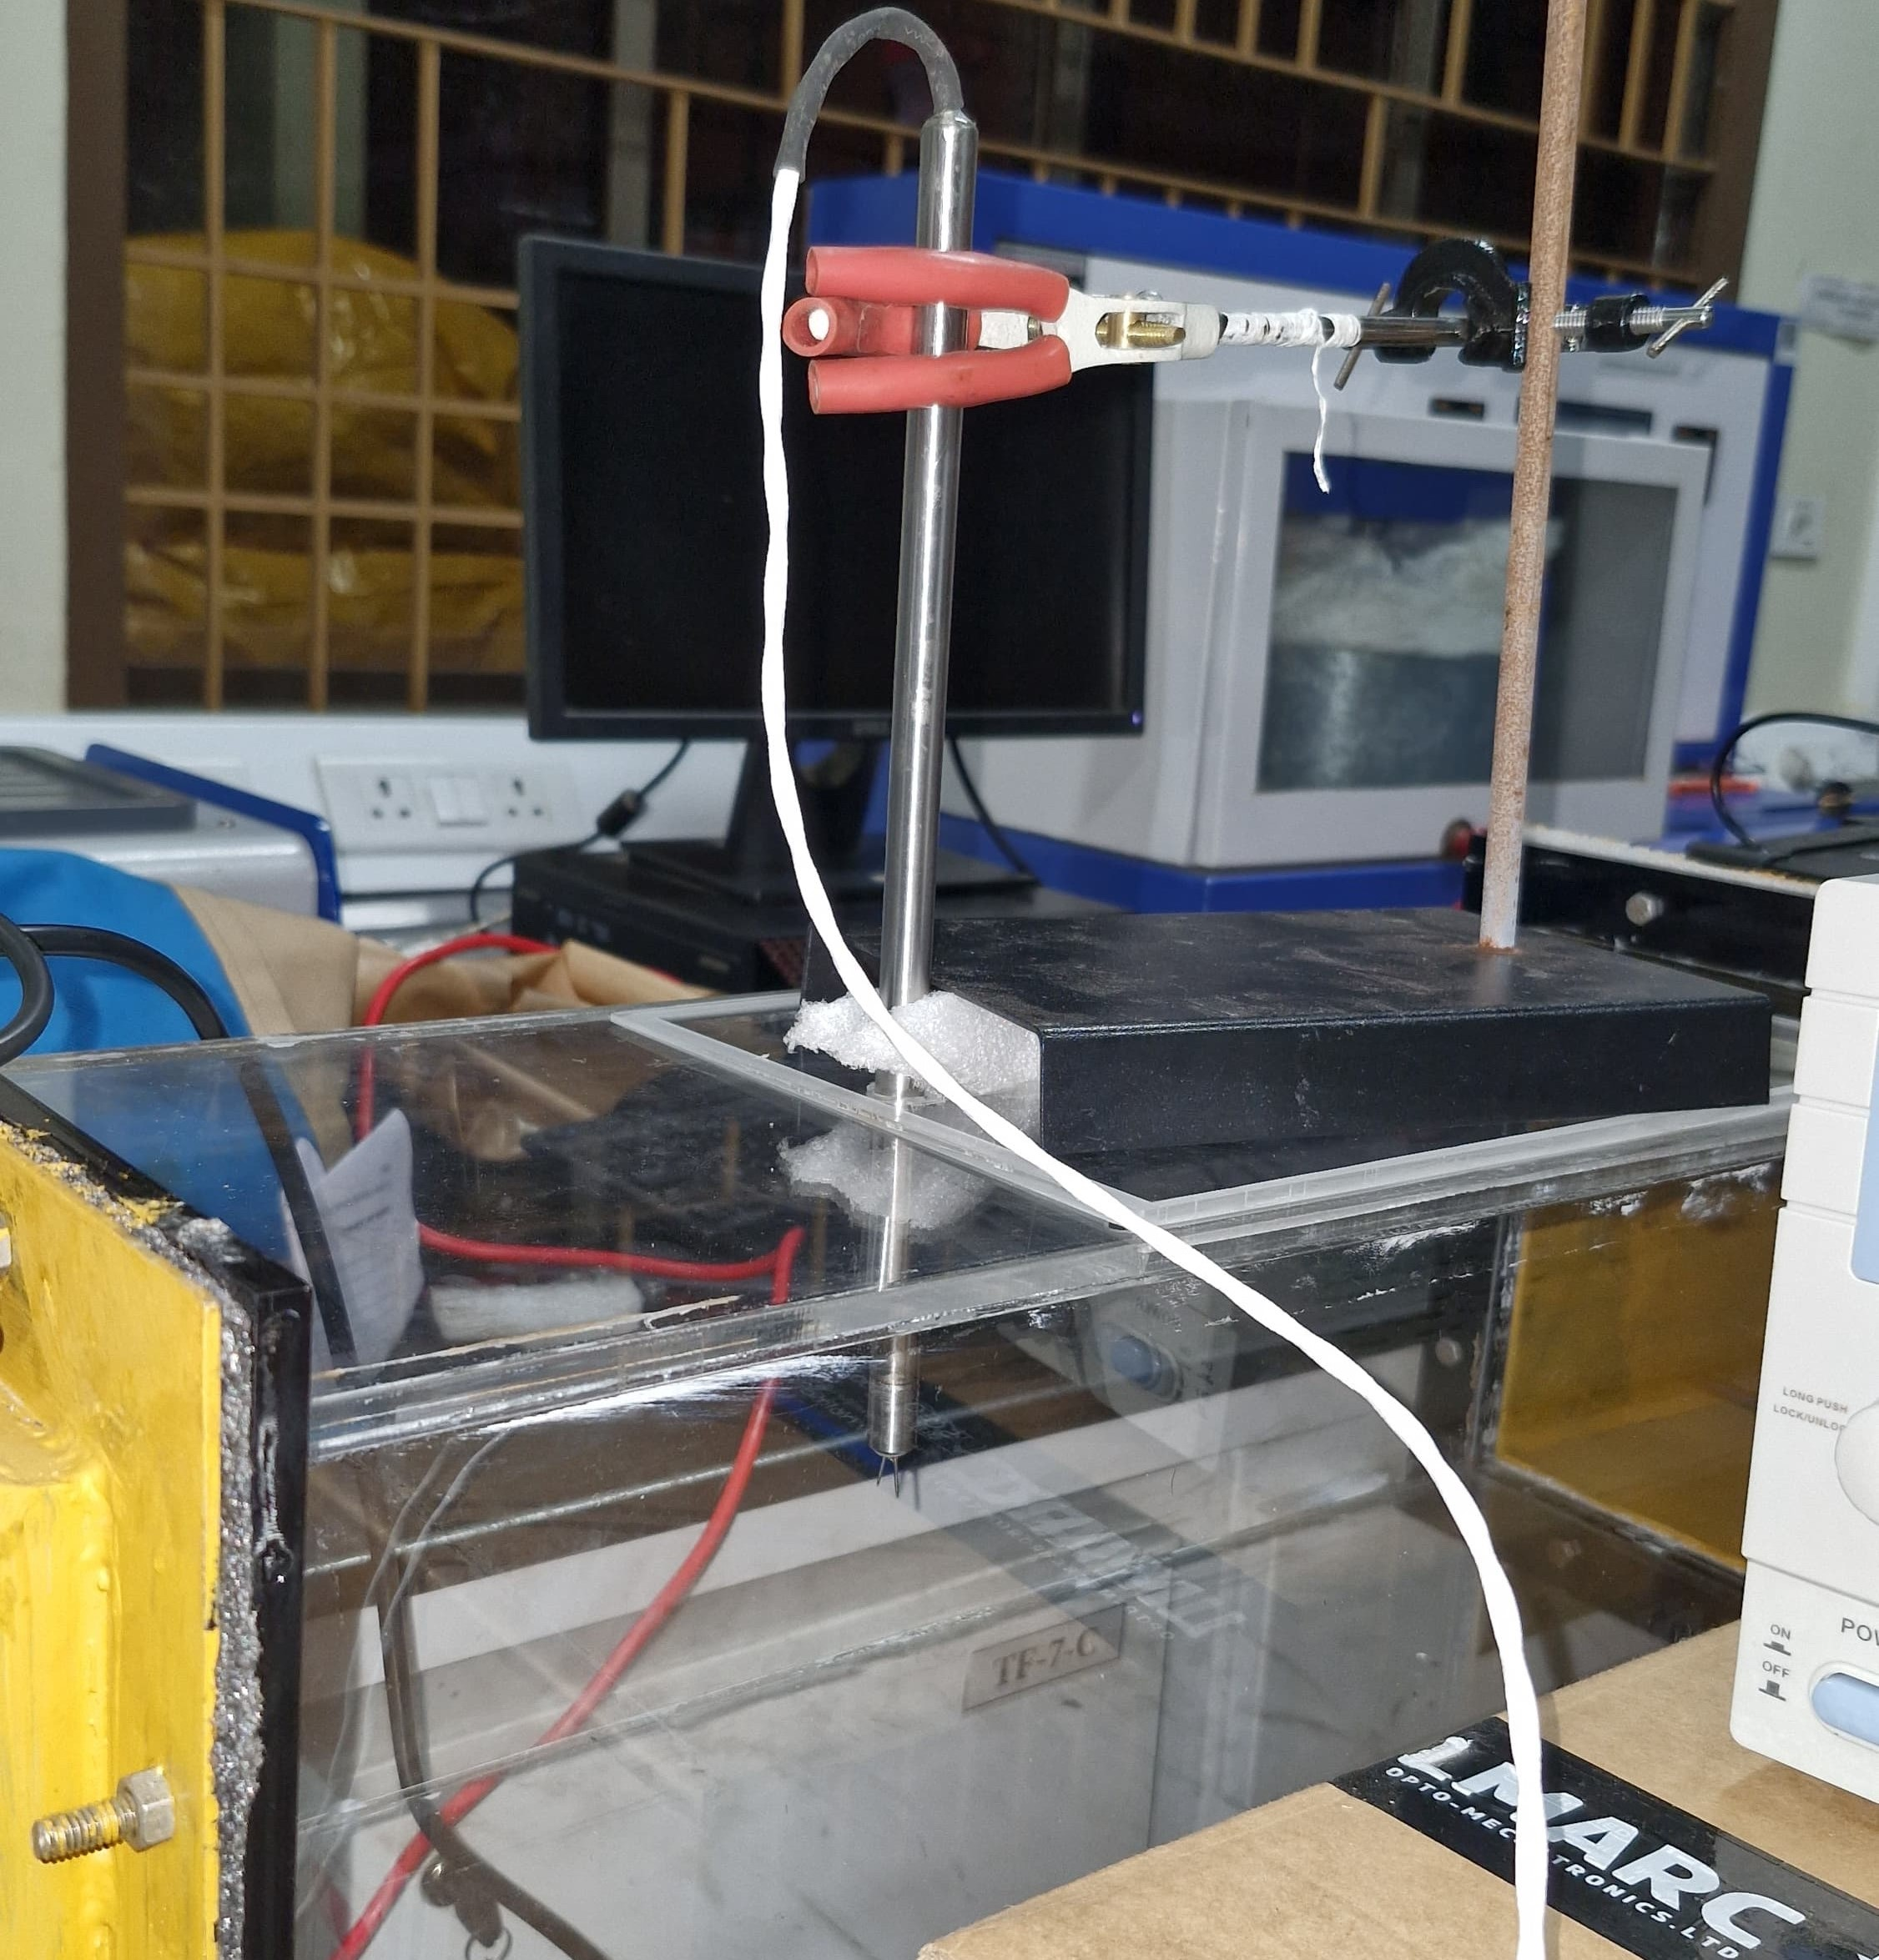
\includegraphics[width=0.5\linewidth]{gfx/HWA_CC_Calibration.jpeg}
%     \caption{Calibration of Hot wire anemometer.}
%     \label{fig:enter-label}
% \end{figure}
In this section, the calibration of the hot wire anemometer is discussed. The calibration procedure is the same as that followed in calibration of the tungsten filament of the bulb. The hot wire anemometer is kept at the middle of the wind tunnel and a constant current of 0.1~A is supplied (see Fig.~\ref{fig:calibration_HWA}). Since the diameter of the hot wire is 10 $\mu$ the current input is restricted to 0.1 A, which avoids the red hot condition of the hot wire and also oxidation. The output of the hot wire anemometer is recorded for 5~s without any flow which gives the no flow voltage. Further, the speed of the suction fan is slowly increased, and the corresponding output voltage is measured. The hot wire anemometer output voltage is recorded for a pitot tube pressure of 1~Pa, 2~Pa, 3~Pa, 4~Pa, 6~Pa, 9~Pa. The flow velocity can be calculated using Eq.~(\ref{eq:press_vel equation}). The differential pressure, velocity and corresponding voltage output of the filament is given in Table~\ref{tab:output_hwa}.
\begin{figure}[ht]
    \centering
    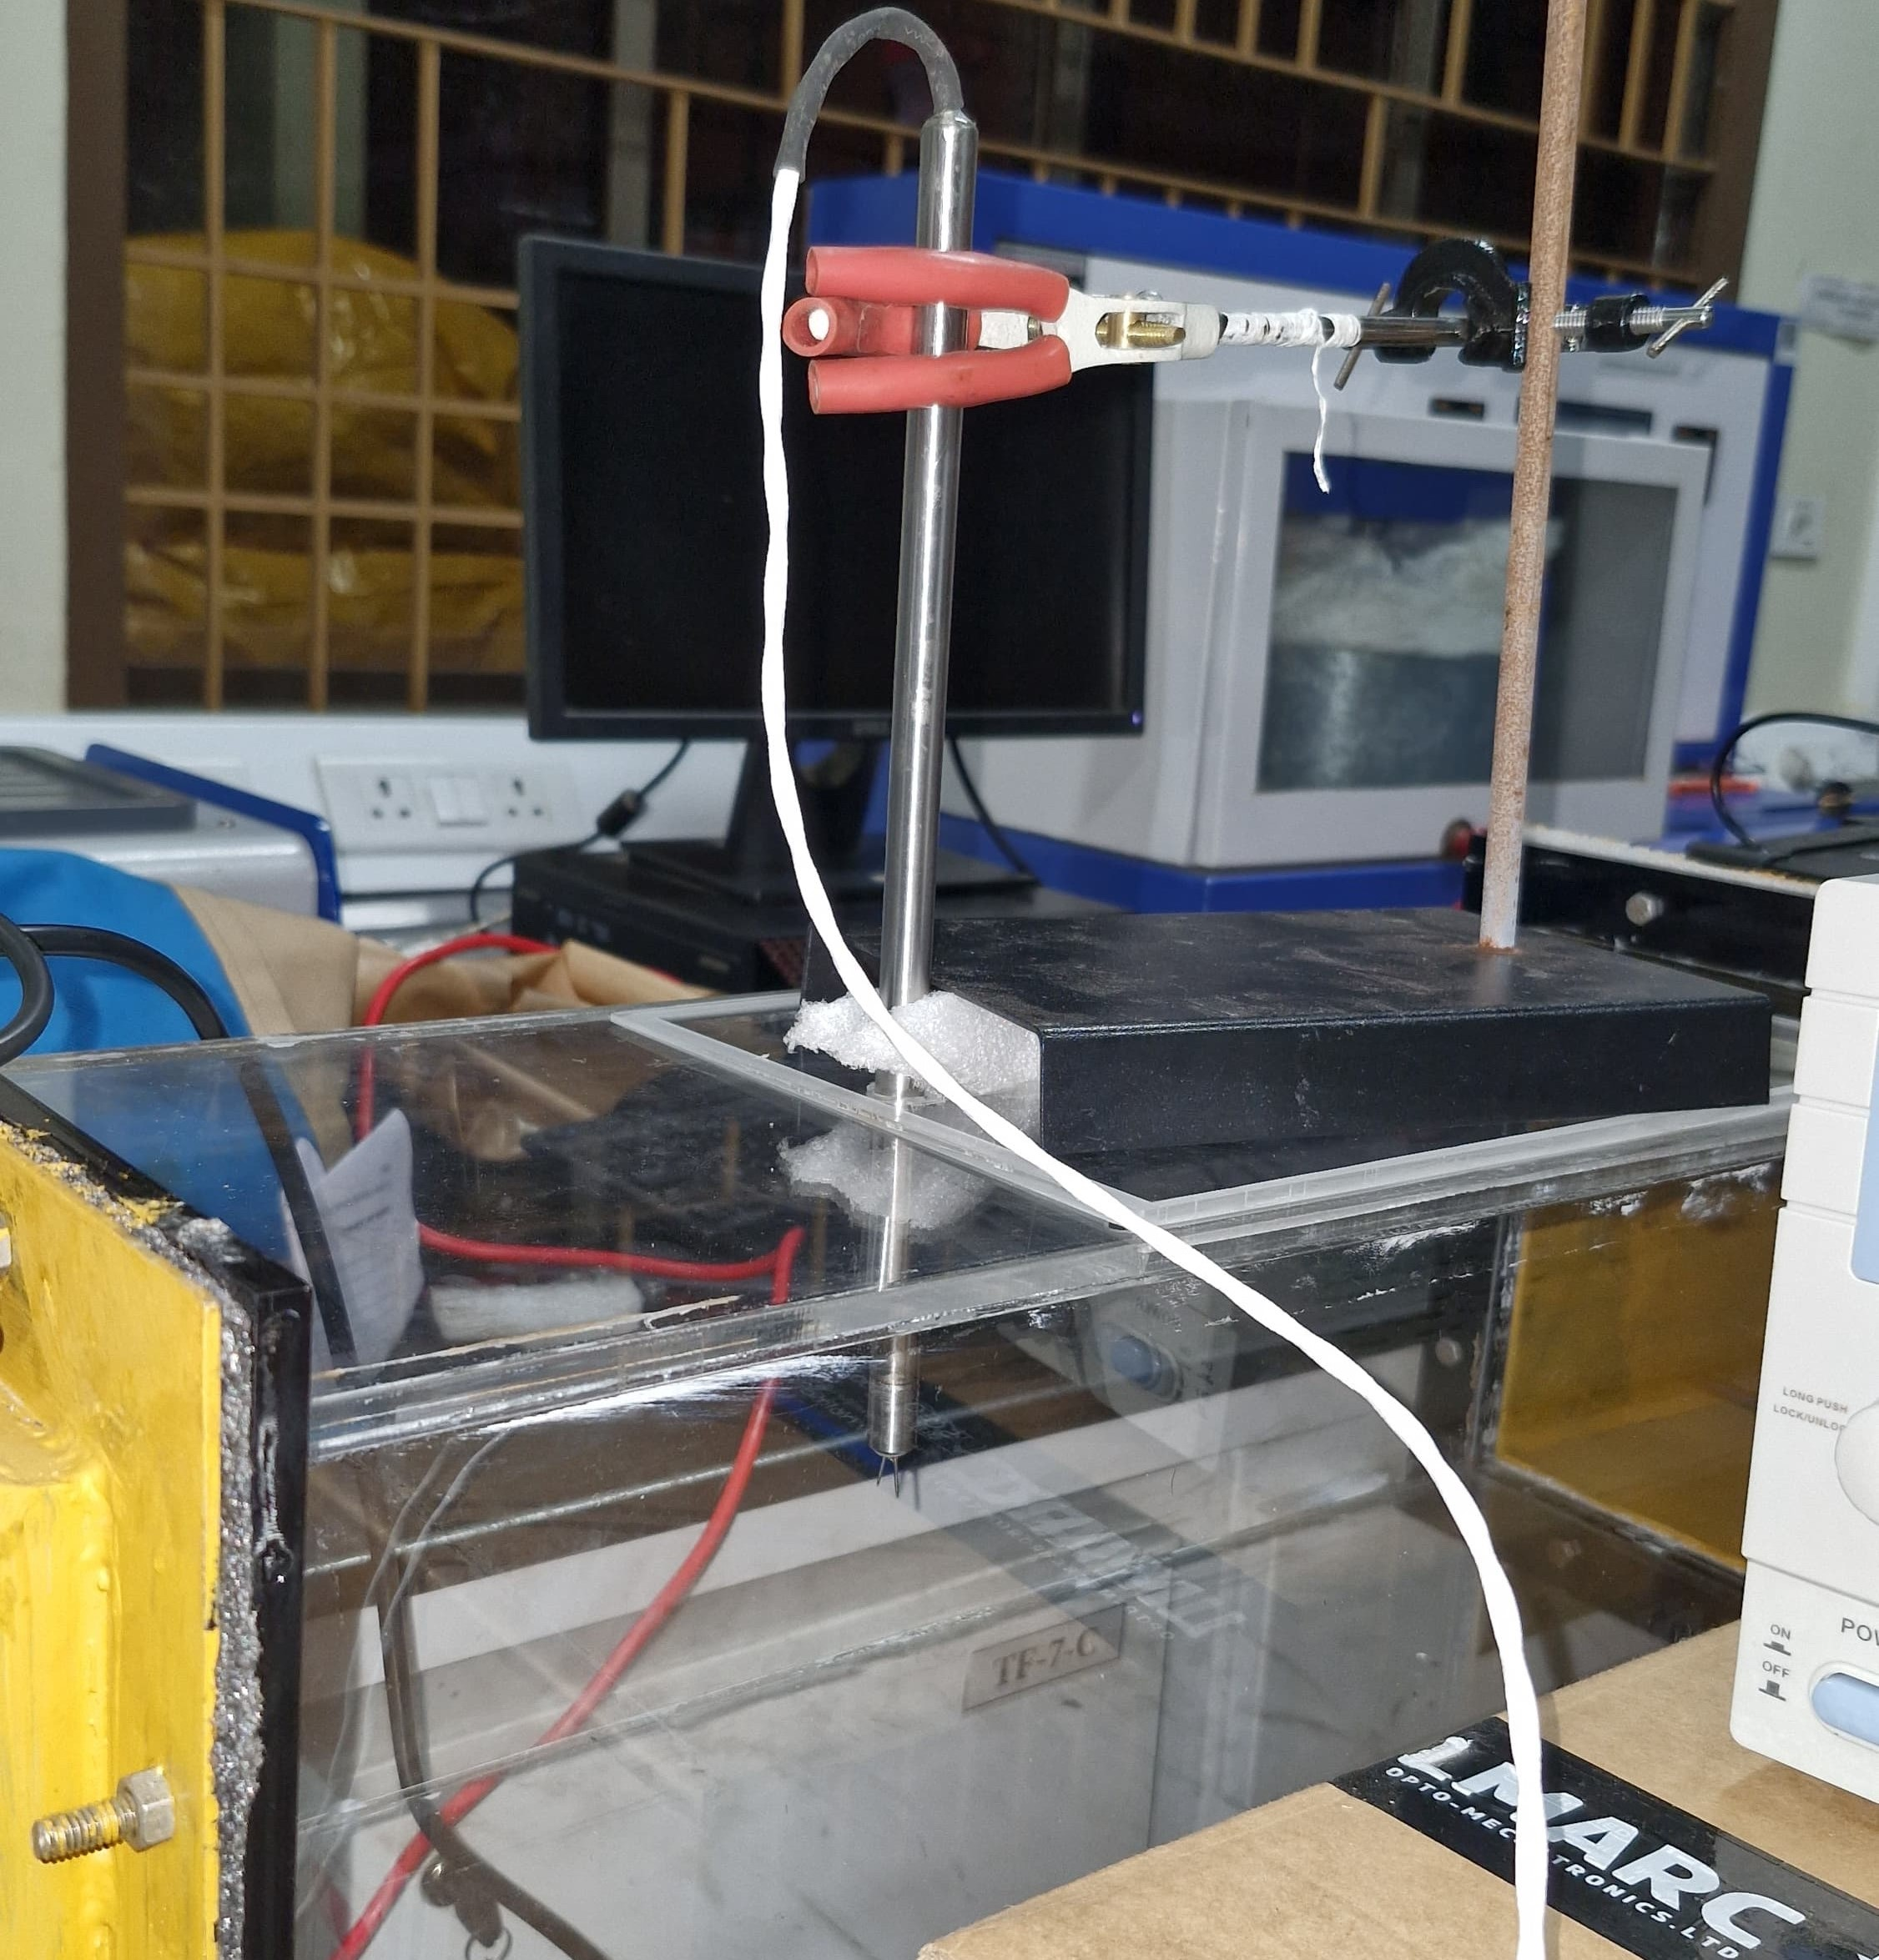
\includegraphics[width=0.5\linewidth]{gfx/HWA_CC_Calibration.jpeg}
    \caption{Calibration of hot wire anemometer.}
    \label{fig:calibration_HWA}
\end{figure}
\begin{table}[ht]
$E_0 = 1.316~V$
\centering
    \caption{The flow velocity and the output mean voltage of the hot wire anemometer.}
    \begin{tabular}{|c|c|c|}
    \toprule
       \textbf{Differential Pressure $\Delta P$ (Pa)}  & \textbf{Velocity $U$ (m/s)} & \textbf{Mean Voltage $E$ (Volts)} \\
       \midrule
        1 & 1.307 & 1.002 \\ \hline
        2 & 1.849 & 0.990 \\ \hline
        3 & 2.265 & 0.957 \\ \hline
        4 & 2.615 & 0.933 \\ \hline
        6 & 3.203 & 0.917 \\ \hline
        9 & 3.922 & 0.903 \\ 
        \bottomrule
    \end{tabular}
    \label{tab:output_hwa}
\end{table}

The hot wire anemometer is also calibrated using King's law (Eq.~(\ref{eq:kings law})) and the numerical constants are estimated by the numerical method (method of least squares) using Eq.~(\ref{eq:lin eq 1}) and Eq.~(\ref{eq:lin eq 2}). On solving the equations, the numerical constants $B$ and $n$ are derived as 0.676 and 0.232, respectively. The calibration equation can be written as 
\begin{equation}\label{eq:calib_eqn_hwa}
    E^2 = 1.73 - 0.676\cdot U^{0.232}
\end{equation}
Equation~\ref{eq:calib_eqn_hwa} is used to calculate the voltage for different velocities and the error between measured and calculated voltage is given in Table~\ref{tab:error_hwa}.
\begin{table}[H]
    \centering
    \caption{The difference of calibrated voltage from measured voltage for hot wire anemometer.}
    \begin{tabular}{|c|c|c|c|}
    \toprule
         Measured $E^2$& Calculated $E^2$ & Error & Error$^2$\\
         \midrule
          1.004 & 1.013 & 0.009 & 8.70$\times$ 10$^{-5}$ \\ \hline
          0.981 & 0.953 & 0.027 & 7.45$\times$ 10$^{-5}$ \\ \hline
          0.917 & 0.916 & 0.001 & 3.72$\times$ 10$^{-5}$ \\ \hline
          0.870 & 0.888 & -0.018 & 3.34$\times$ 10$^{-4}$ \\ \hline
          0.841 & 0.848 & -0.007 & 4.84$\times$ 10$^{-5}$ \\ \hline
          0.815 & 0.805 & 0.010 & 9.2$\times$ 10$^{-5}$  \\
         \bottomrule
         
    \end{tabular}
    \label{tab:error_hwa}
\end{table}
The comparison of the variation of the measured voltage and the calculated voltage with the velocity is given in Fig.~\ref{fig:calibration_of_hwa}

\begin{figure}[ht]
    \centering
    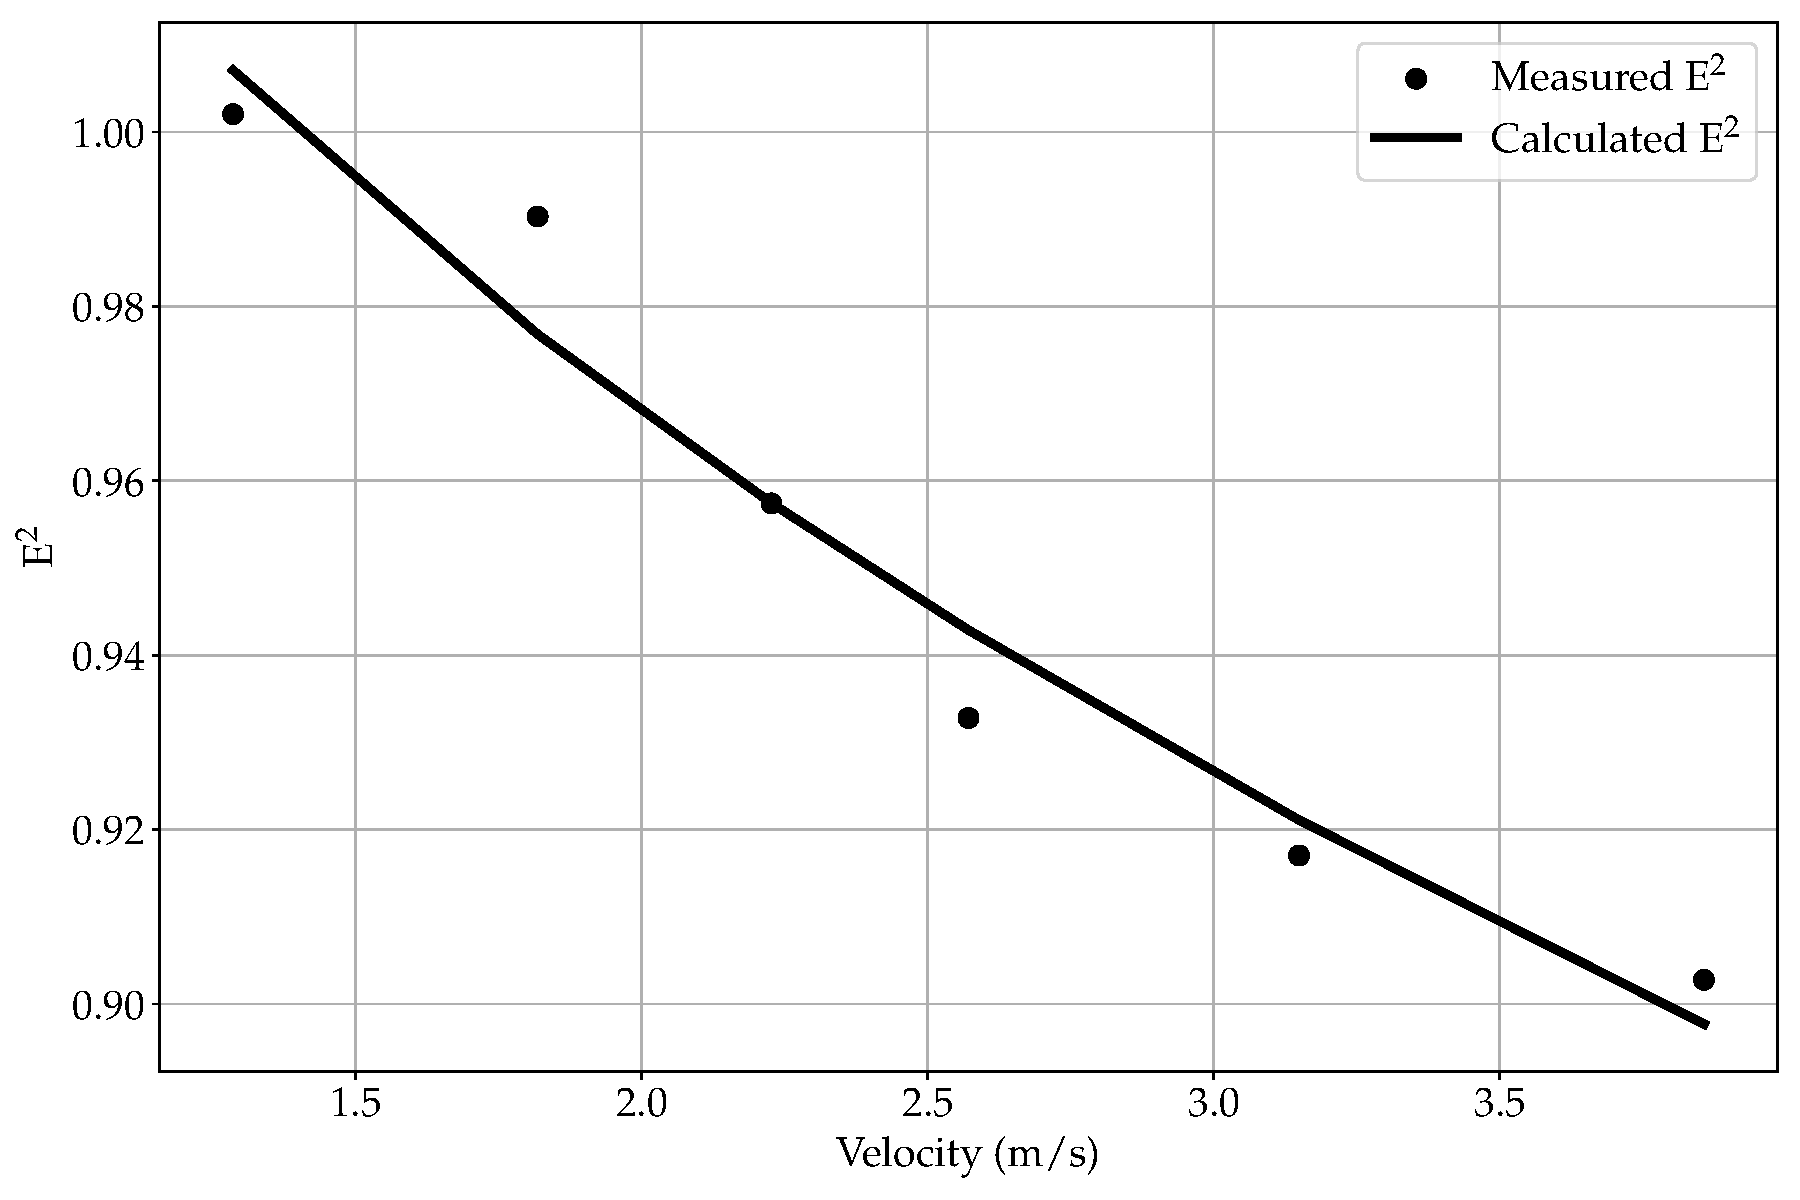
\includegraphics[width=\linewidth]{gfx/calibration_of_hot_wire.pdf}
    \caption{Comparison of measured and calculated voltage of the hot wire anemometer}
    \label{fig:calibration_of_hwa}
\end{figure}
\begin{figure}[H]
    \centering
    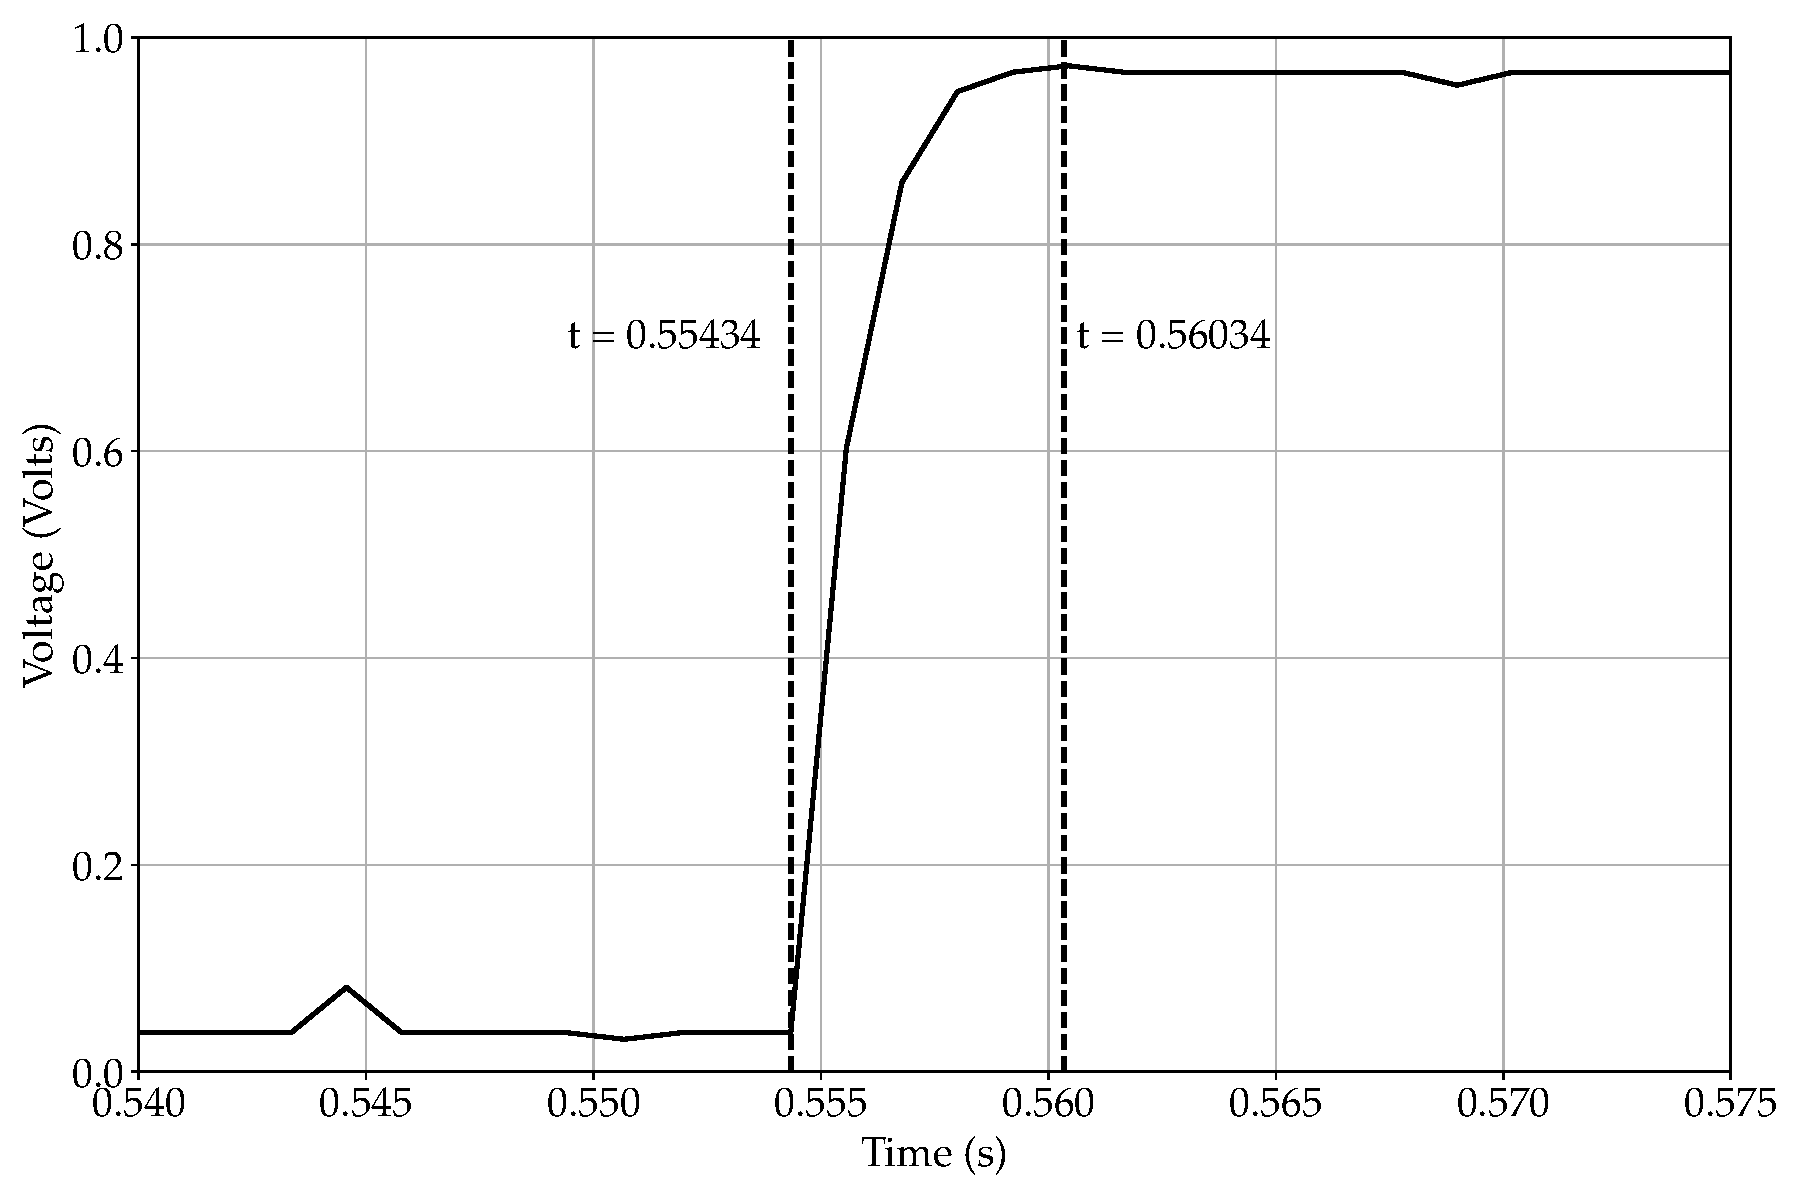
\includegraphics[width=\linewidth]{gfx/Time_constant_hot_wire.pdf}
    \caption{Response of a hot wire anemometer for a step input.}
    \label{fig:time_hotwire}
\end{figure}
\section{Time constant of the hot wire anemometer}
The time constant $\tau$ of the hot wire anemometer is also estimated by providing a step input to it and recording the output in the oscilloscope. Fig.~\ref{fig:time_hotwire} shows the variation of output voltage with time when a step input is given to the anemometer. It can be seen that the hot wire anemometer takes about 6~ms to give steady output.



\section{Chapter summary}

In this chapter, the calibration of the bulb filament and the hot-wire anemometer are discussed. The estimation of time constant is also discussed. It is observed that the time constant of the hot wire anemometer is much (75 times) less than the filament of the bulb. So, it can be concluded that for further analysis in the wind tunnel, the hot wire anemometer is better than the bulb filament. In the next chapter, the vortex analysis in the wind tunnel performed using the hot wire anemometer is discussed.